% \documentclass[aspectratio=169,notes]{beamer}
\documentclass[aspectratio=169]{beamer}
\usetheme[faculty=phil]{fibeamer}
\usepackage{polyglossia}
\setmainlanguage{english} %% main locale instead of `english`, you
%% can typeset the presentation in either Czech or Slovak,
%% respectively.
\setotherlanguages{russian} %% The additional keys allow
%%
%%   \begin{otherlanguage}{czech}   ... \end{otherlanguage}
%%   \begin{otherlanguage}{slovak}  ... \end{otherlanguage}
%%
%% These macros specify information about the presentation
\title[Introduction to Robotics (In2Ro)]{Introduction to Robotics, Lecture 3} %% that will be typeset on the
\subtitle{Differential Kinematics 
\\ Joint and tool velocities \\ Jacobians and inverse differential maps  } %% title page.
\author{Oleg Bulichev}
%% These additional packages are used within the document:
\usepackage{ragged2e}  % `\justifying` text
\usepackage{booktabs}  % Tables
\usepackage{tabularx}
\usepackage{tikz}      % Diagrams
\usetikzlibrary{calc, shapes, backgrounds, trees, positioning, arrows.meta}
\usetikzlibrary{decorations.pathreplacing,calligraphy,calc,graphs}
\usepackage{amsmath, amssymb}
\usepackage{url}       % `\url`s
\usepackage{listings}  % Code listings
\usepackage{floatrow}
\usepackage{subcaption}
\usepackage{mathtools}
\usepackage{todonotes}
\usepackage{fontspec}
\usepackage{multicol}
\usepackage{pdfpages}
\usepackage{wrapfig}
\usepackage{qrcode}
\usepackage{animate}
\usepackage{booktabs}
\usepackage{multirow}
\usepackage{graphicx}
\usepackage{colortbl}

\graphicspath{{resources/}}
\frenchspacing

\setbeamertemplate{caption}{\raggedright\insertcaption\par}
\usetikzlibrary{graphs}

% \usepackage[backend=biber,style=ieee,autocite=footnote]{biblatex}
% \addbibresource{biblio.bib}
% \DefineBibliographyStrings{english}{%
%   bibliography = {References},}

\newcommand{\oleg}[2][] {\todo[color=red, #1] {OLEG:\\ #2}}
\newcommand{\fbckg}[1]{\usebackgroundtemplate{\includegraphics[width=\paperwidth]{#1}}}%frame background

\usepackage[framemethod=TikZ]{mdframed}
\newcommand{\dbox}[1]{
\begin{mdframed}[roundcorner=3pt, backgroundcolor=yellow, linewidth=0]
\vspace{1mm}
{#1}
\vspace{1mm}
\end{mdframed}
}

\begin{document}
\setlength{\abovedisplayskip}{0pt}
\setlength{\belowdisplayskip}{0pt}
\setlength{\abovedisplayshortskip}{0pt}
\setlength{\belowdisplayshortskip}{0pt}

\fbckg{fibeamer/figs/title_page.png}
\frame[c]{\setcounter{framenumber}{0}
    \usebeamerfont{title}%
    \usebeamercolor[fg]{title}%
    \begin{minipage}[b][6.5\baselineskip][b]{\textwidth}%
        \textcolor{black}{\raggedright\inserttitle}
    \end{minipage}
    % \vskip-1.5\baselineskip

    \usebeamerfont{subtitle}%
    \usebeamercolor[fg]{framesubtitle}%
    \begin{minipage}[b][3\baselineskip][b]{\textwidth}
        \raggedright%
        \insertsubtitle%
    \end{minipage}
    \vskip.25\baselineskip
}

\fbckg{fibeamer/figs/common.png}

\begin{frame}[t]{Where This Lecture Starts}
    \framesubtitle{Pose maps are nonlinear; the velocity map is linear at a frozen configuration}
    \begin{columns}[T,onlytextwidth]
        \begin{column}{0.48\textwidth}
            \centering
            \begin{tikzpicture}[node distance=8mm, every node/.style={draw, rounded corners, align=center, minimum width=28mm, minimum height=7mm}]
                \node (q) {Joint coordinates\\$q$};
                \node[right=of q] (x) {Task coordinates\\$X$};
                \draw[-{Latex}] (q) -- node[above,draw=none,minimum width=0] {$\mathrm{FK}$} (x);
                \draw[-{Latex}] (x) to[bend left=35] node[below,draw=none,minimum width=0] {$\mathrm{IK}$} (q);
            \end{tikzpicture}
        \end{column}
        \begin{column}{0.48\textwidth}
            \centering
            \begin{tikzpicture}[node distance=8mm, every node/.style={draw, rounded corners, align=center, minimum width=28mm, minimum height=7mm}]
                \node (qd) {Joint rates\\$\dot q$};
                \node[right=of qd] (xd) {Task rates\\$\dot X$};
                \draw[-{Latex}] (qd) -- node[above,draw=none,minimum width=0] {$J(q)$} (xd);
            \end{tikzpicture}
            \[
                \dot X=J(q)\dot q
            \]
            At a fixed $q$, the map is linear in $\dot q$; moving $q$ changes the map itself.
        \end{column}
    \end{columns}
\end{frame}

\begin{frame}[t]{What Differential Kinematics Is}
    \framesubtitle{Instantaneous motion connects joint-space rates to linear and angular task motion}
    \begin{itemize}
        \item Differential kinematics relates joint motion to end-effector linear and angular motion.
        \item The mapping is instantaneous: it is evaluated at one configuration, not over an entire path.
        \item Differentiate direct kinematics in time, or construct the map geometrically from joint axes.
        \item Rotation is the subtle part: coordinate rates and angular velocity are not generally the same quantity.
    \end{itemize}
\end{frame}

\begin{frame}[t]{Angular Velocity of a Rigid Body}
    \framesubtitle{Rigidity makes one angular velocity serve every point of the same body}
    \begin{columns}[T,onlytextwidth]
        \begin{column}{0.49\textwidth}
            \centering
            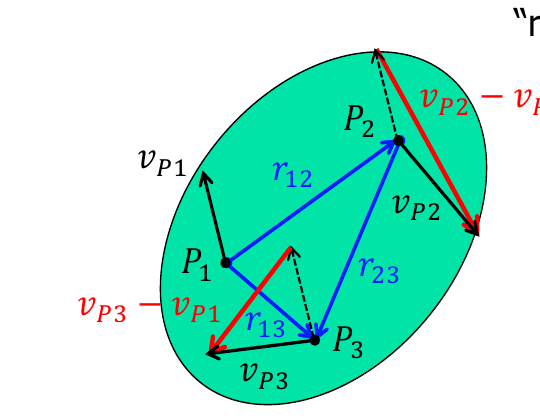
\includegraphics[width=\linewidth,height=0.59\textheight,keepaspectratio]{deluca11_p003_rigidbody.png}
        \end{column}
        \begin{column}{0.47\textwidth}
            Every inter-point distance is fixed:
            \[
                \|r_{ij}\|=\text{const}
                \quad\Rightarrow\quad
                v_{P_i}-v_{P_j}\perp r_{ij}.
            \]
            Writing this condition for three points forces the pairwise angular rates to agree:
            \[
                \omega_1=\omega_2=\omega.
            \]
            A rigid body has one angular velocity, not one for every pair of points.
        \end{column}
    \end{columns}
\end{frame}

\begin{frame}[t]{The Fundamental Kinematic Equation}
    \framesubtitle{Knowing one point velocity and the body angular velocity determines any other point}
    \[
        v_{P_j}=v_{P_i}+\omega\times r_{ij}
        =v_{P_i}+S(\omega)r_{ij},
        \qquad
        \dot r_{ij}=\omega\times r_{ij}.
    \]
    \begin{block}{Two limiting motions}
        If $\omega=0$, every point has the same velocity: pure translation. If two points are at rest, the body rotates about the line joining them.
    \end{block}
    The matrix $S(\omega)$ is skew-symmetric and represents cross product with $\omega$.
\end{frame}

\begin{frame}[t]{One Joint, One Velocity Contribution}
    \framesubtitle{Revolute and prismatic joints contribute along the axis of their preceding frame}
    \begin{columns}[T,onlytextwidth]
        \begin{column}{0.58\textwidth}
            \centering
            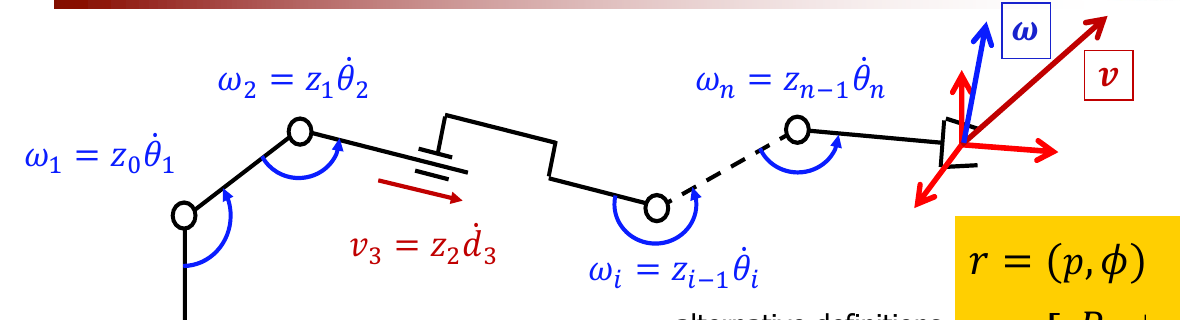
\includegraphics[width=\linewidth,height=0.46\textheight,keepaspectratio]{deluca11_p004_chain.png}
        \end{column}
        \begin{column}{0.38\textwidth}
            \[
                \omega_i=z_{i-1}\dot\theta_i
                \qquad
                v_i=z_{i-1}\dot d_i
            \]
            A revolute joint contributes angular velocity; a prismatic joint contributes linear velocity. Contributions add because $v$ and $\omega$ are vectors.
        \end{column}
    \end{columns}
\end{frame}

\begin{frame}[t]{Why $\omega$ Is Not the Derivative of an Orientation}
    \framesubtitle{Angular velocity is a vector, whereas a minimal orientation triple is a coordinate choice}
    \begin{itemize}
        \item Linear and angular velocities add in any order.
        \item A minimal orientation triple $\phi$ is not a vector: composing rotations is not addition of triples.
        \item Therefore, in general,
        \[
            \omega\neq\dot\phi.
        \]
        \item Both $(p,\phi)$ and a rotation matrix $R$ are valid orientation descriptions; their rates need different treatment.
    \end{itemize}
\end{frame}

\begin{frame}[t]{Translations Always Commute}
    \framesubtitle{The order of two displacements does not affect the final position}
    \begin{columns}[T,onlytextwidth]
        \begin{column}{0.61\textwidth}
            \centering
            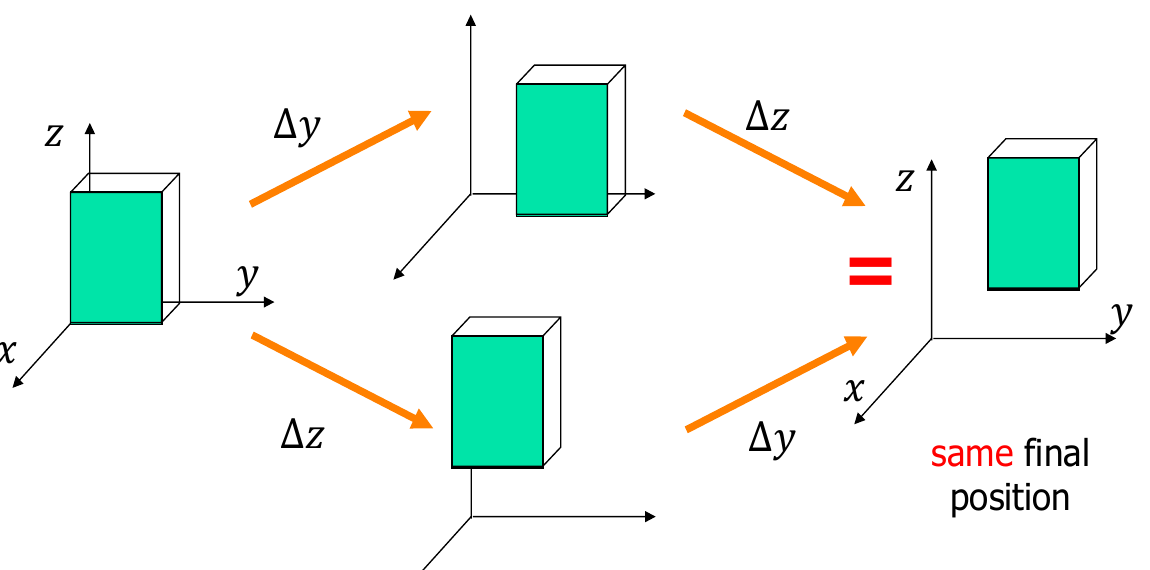
\includegraphics[width=\linewidth,height=0.60\textheight,keepaspectratio]{deluca11_p005_translations.png}
        \end{column}
        \begin{column}{0.35\textwidth}
            \[
                \Delta y\ \text{then}\ \Delta z
                =\Delta z\ \text{then}\ \Delta y.
            \]
            Finite and infinitesimal displacements both add as vectors; no ordering bookkeeping is needed.
        \end{column}
    \end{columns}
\end{frame}

\begin{frame}[t]{Finite Rotations Do Not Commute}
    \framesubtitle{Changing the order of rotations about different axes changes the final orientation}
    \begin{columns}[T,onlytextwidth]
        \begin{column}{0.64\textwidth}
            \centering
            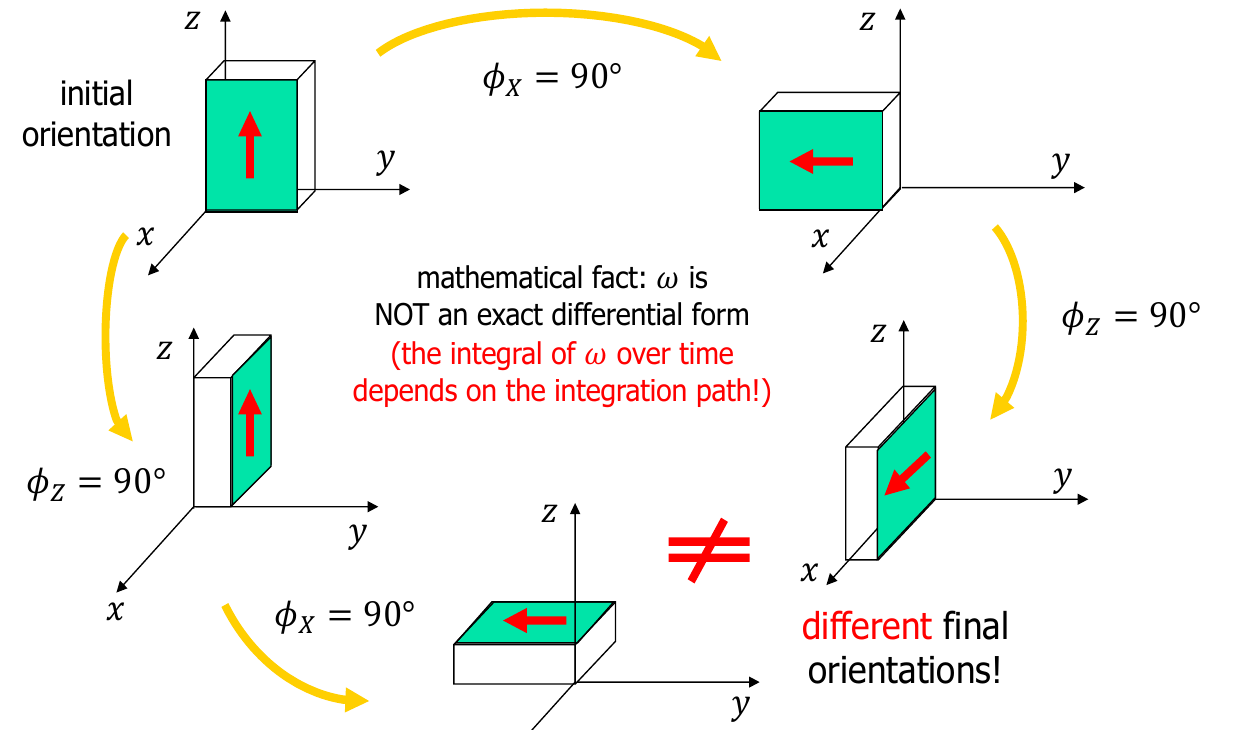
\includegraphics[width=\linewidth,height=0.62\textheight,keepaspectratio]{deluca11_p006_rotations.png}
        \end{column}
        \begin{column}{0.32\textwidth}
            \[
                R_X(\pi/2)R_Z(\pi/2)
            \]
            \[
                \neq R_Z(\pi/2)R_X(\pi/2).
            \]
            Rotations about one fixed axis are the special commuting case.
        \end{column}
    \end{columns}
\end{frame}

\begin{frame}[t]{$\omega$ Is Not an Exact Differential}
    \framesubtitle{Equal axis-wise areas of angular-rate profiles can lead to different orientations}
    \begin{columns}[T,onlytextwidth]
        \begin{column}{0.48\textwidth}
            Two rate profiles can satisfy
            \[
                \int_0^T\omega\,dt
            \]
            with the same vector result while producing different final rotation matrices $R_f$. The integral depends on the path through orientation space.
        \end{column}
        \begin{column}{0.48\textwidth}
            Coordinate rates are different:
            \[
                \int_0^T\dot\phi\,dt=\phi_f-\phi_i.
            \]
            This telescopes because $\dot\phi$ is an exact differential of its chosen coordinates.
        \end{column}
    \end{columns}
\end{frame}

\begin{frame}[t]{Infinitesimal Rotations Do Commute}
    \framesubtitle{Keeping only first-order terms recovers an additive differential description}
    \[
        R(d\phi)=I+S(d\phi),
        \qquad
        S(d\phi)=
        \begin{bmatrix}
            0&-d\phi_Z&d\phi_Y\\
            d\phi_Z&0&-d\phi_X\\
            -d\phi_Y&d\phi_X&0
        \end{bmatrix}.
    \]
    Multiplying elementary infinitesimal rotations in any order gives the same first-order matrix. Products of two small increments are discarded, not assumed to be zero.
\end{frame}

\begin{frame}[t]{Time Derivative of a Rotation Matrix}
    \framesubtitle{A matrix derivative reveals angular velocity without choosing orientation angles}
    Orthogonality gives a skew-symmetric product:
    \[
        \dot R R^{T}=S,
        \qquad S=S(\omega).
    \]
    Hence
    \[
        \dot R=S(\omega)R
        \qquad\Longleftrightarrow\qquad
        S(\omega)=\dot R R^{T}.
    \]
    This is the matrix form of angular velocity and will later extract the angular part of a Jacobian column.
\end{frame}

\begin{frame}[t]{Worked Example: Differentiating an Elementary Rotation}
    \framesubtitle{For a rotation about $x$, the matrix identity returns the expected axis velocity}
    \[
        R_X(\phi)=
        \begin{bmatrix}1&0&0\\0&\cos\phi&-\sin\phi\\0&\sin\phi&\cos\phi\end{bmatrix}
        \quad\Rightarrow\quad
        \dot R_XR_X^T=
        \begin{bmatrix}0&0&0\\0&0&-\dot\phi\\0&\dot\phi&0\end{bmatrix}.
    \]
    \[
        \omega=\dot\phi\begin{bmatrix}1\\0\\0\end{bmatrix}.
    \]
    More generally, an axis--angle rotation $R(r,\theta)$ has $\omega=\dot\theta r$ when its axis is fixed.
\end{frame}

\begin{frame}[t]{RPY Rates Against Angular Velocity}
    \framesubtitle{A coordinate singularity, not a robot singularity}
    \begin{columns}[T,onlytextwidth]
        \begin{column}{0.42\textwidth}
            \centering
            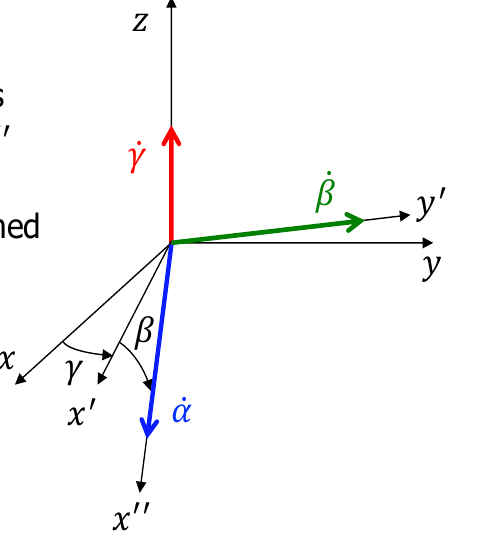
\includegraphics[width=\linewidth,height=0.46\textheight,keepaspectratio]{deluca11_p011_rpyaxes.png}
        \end{column}
        \begin{column}{0.54\textwidth}
            \small
            The Z, new-Y, and newer-X rotation axes form the columns of $T_{\mathrm{RPY}}$:
            \[
                \omega=T_{\mathrm{RPY}}(\beta,\gamma)
                \begin{bmatrix}\dot\alpha\\\dot\beta\\\dot\gamma\end{bmatrix}.
            \]
            Its determinant is $\det T_{\mathrm{RPY}}=\cos\beta$. At $\beta=\pm\pi/2$, this representation cannot express every angular velocity by angle rates.
        \end{column}
    \end{columns}
\end{frame}

\begin{frame}[t]{Two Jacobians, Not One}
    \framesubtitle{Analytic and geometric Jacobians answer different instantaneous questions}
    \begin{columns}[T,onlytextwidth]
        \begin{column}{0.48\textwidth}
            \begin{block}{Analytic Jacobian}
                For task coordinates $r=f_r(q)$,
                \[
                    \dot r=\frac{\partial f_r}{\partial q}\dot q
                    =J_r(q)\dot q.
                \]
                It is obtained by differentiating the task map.
            \end{block}
        \end{column}
        \begin{column}{0.48\textwidth}
            \begin{block}{Geometric Jacobian}
                \[
                    \begin{bmatrix}v\\\omega\end{bmatrix}
                    =\begin{bmatrix}J_L(q)\\J_A(q)\end{bmatrix}\dot q
                    =J(q)\dot q.
                \]
                It maps to the physical end-effector twist.
            \end{block}
        \end{column}
    \end{columns}
    Their lower halves differ because $\omega\neq\dot\phi$ in general.
\end{frame}

\begin{frame}[t]{The Jacobian Equation}
    \framesubtitle{Each entry is a local sensitivity, and the matrix changes with configuration}
    \[
        \dot X_{6\times1}=J_{6\times n}(q)\dot q_{n\times1},
        \qquad
        J=\left[\frac{\partial f_i}{\partial q_j}\right]_{
        \substack{i=1,\ldots,6\\j=1,\ldots,n}}.
    \]
    \begin{itemize}
        \item A six-quantity task and a seven-joint robot give a $6\times7$ Jacobian.
        \item $J(q)$ is recomputed at every configuration; it is not a constant robot property.
        \item Column $j$ records the effect of moving only joint $j$ at that configuration.
    \end{itemize}
\end{frame}

\begin{frame}[t]{Which Vector Is on the Left?}
    \framesubtitle{Coordinate rates use the analytic Jacobian; physical twist uses the geometric Jacobian}
    \begin{columns}[T,onlytextwidth]
        \begin{column}{0.48\textwidth}
            \begin{block}{Coordinate-rate output}
                \[
                    \begin{bmatrix}\dot p\\\dot\phi\end{bmatrix}
                    =J_r(q)\dot q.
                \]
                The partial-derivative array is correct for the stack $(\dot p,\dot\phi)$.
            \end{block}
        \end{column}
        \begin{column}{0.48\textwidth}
            \begin{block}{Physical-twist output}
                \[
                    \begin{bmatrix}v\\\omega\end{bmatrix}
                    =J(q)\dot q.
                \]
                Here $\omega$ is not the derivative of three orientation coordinates.
            \end{block}
        \end{column}
    \end{columns}
    \[
        \begin{bmatrix}v\\\omega\end{bmatrix}
        =\operatorname{blkdiag}(I,T(\phi))
        \begin{bmatrix}\dot p\\\dot\phi\end{bmatrix}.
    \]
\end{frame}

\begin{frame}[t]{A Jacobian Is a Linear Map Between Two Spaces}
    \framesubtitle{The same configuration-dependent map appears in velocity, statics, and stiffness models}
    \begin{columns}[T,onlytextwidth]
        \begin{column}{0.31\textwidth}
            \begin{block}{Motion}
                Small joint displacements map to small Cartesian displacements.
            \end{block}
        \end{column}
        \begin{column}{0.31\textwidth}
            \begin{block}{Statics}
                \[
                    \tau=J^T(q)F.
                \]
                Forces and moments map back to joint torques.
            \end{block}
        \end{column}
        \begin{column}{0.31\textwidth}
            \begin{block}{Stiffness}
                Joint and Cartesian stiffness are related locally through the same geometry.
            \end{block}
        \end{column}
    \end{columns}
    The underlying kinematics is nonlinear, but its local linear map is enough for small changes at one $q$.
\end{frame}

\begin{frame}[t]{Physical Meaning of One Column}
    \framesubtitle{A column asks how the pose changes when only one joint moves}
    \begin{columns}[T,onlytextwidth]
        \begin{column}{0.53\textwidth}
            \small
            For the vertical base axis in the illustrated arm,
            \[
                J_1=
                \begin{bmatrix}
                    -(L_3+L_6)\sin q_1\\
                    (L_3+L_6)\cos q_1\\
                    0\\0\\0\\1
                \end{bmatrix}.
            \]
            It sweeps the end effector in $x$ and $y$, gives no vertical motion or tool tilt, and turns the tool about $z$.
        \end{column}
        \begin{column}{0.43\textwidth}
            \centering
            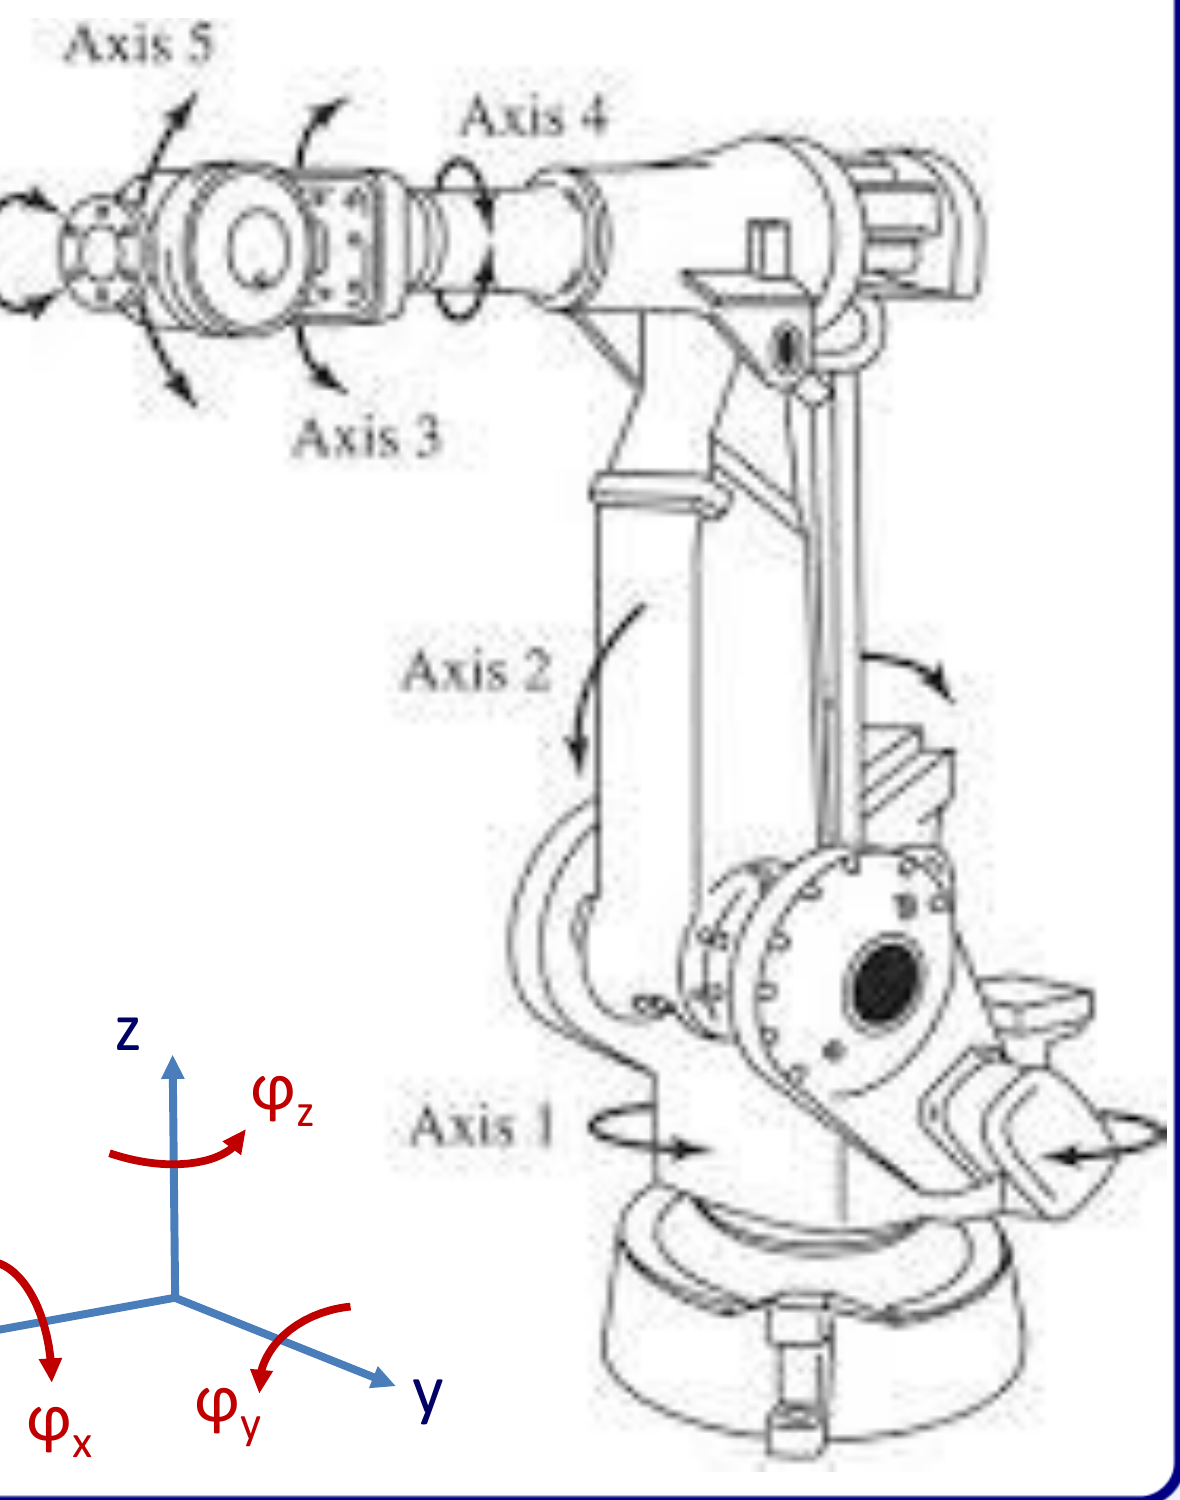
\includegraphics[width=\linewidth,height=0.54\textheight,keepaspectratio]{klimchik_l3_p010_arm.png}
        \end{column}
    \end{columns}
\end{frame}

\begin{frame}[t]{Classical Approach: Differentiate the Direct Kinematics}
    \framesubtitle{For the planar 2R arm, the task coordinates are explicit functions of two angles}
    \begin{columns}[T,onlytextwidth]
        \begin{column}{0.43\textwidth}
            \centering
            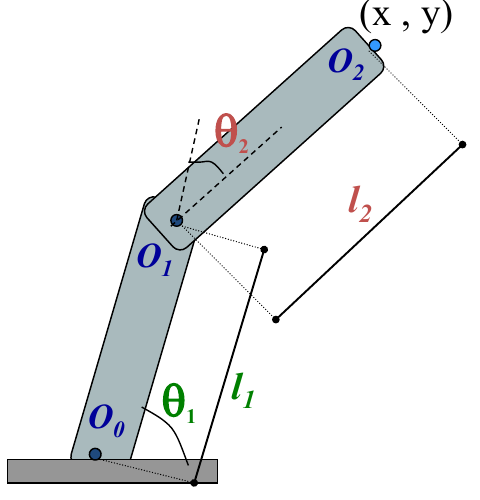
\includegraphics[width=\linewidth,height=0.59\textheight,keepaspectratio]{klimchik_l3_p011_2r.png}
        \end{column}
        \begin{column}{0.53\textwidth}
            \[
                x=l_1c_1+l_2c_{12},\qquad
                y=l_1s_1+l_2s_{12},
            \]
            \[
                \varphi=\theta_1+\theta_2,
                \qquad
                J=\frac{\partial(x,y,\varphi)}{\partial(\theta_1,\theta_2)}.
            \]
            Differentiating column one means following both links; differentiating column two follows the second link only.
        \end{column}
    \end{columns}
\end{frame}

\begin{frame}[t]{The 2R Analytic Jacobian, Evaluated}
    \framesubtitle{The chain rule makes the first column contain the contribution of both links}
    \[
        J=
        \begin{bmatrix}
            -l_1s_1-l_2s_{12} & -l_2s_{12}\\
            l_1c_1+l_2c_{12} & l_2c_{12}\\
            1&1
        \end{bmatrix}.
    \]
    \begin{block}{Read the columns physically}
        Changing $\theta_1$ moves both links, whereas changing $\theta_2$ moves only link 2. The last row is all ones because the tool angle is the sum of the two joint angles.
    \end{block}
\end{frame}

\begin{frame}[t]{Geometric Rule: Columns from Joint Axes}
    \framesubtitle{A column can be built directly from the relevant axis and the tool moment arm}
    \[
        J_i=
        \begin{cases}
        \begin{bmatrix}z_{i-1}\times(o_n-o_{i-1})\\z_{i-1}\end{bmatrix}, & \text{revolute joint},\\[4mm]
        \begin{bmatrix}z_{i-1}\\0\end{bmatrix}, & \text{prismatic joint}.
        \end{cases}
    \]
    Here $z_{i-1}$ is the third column and $o_{i-1}$ the translation column of ${}^{0}T_{i-1}$. A prismatic joint has no angular contribution; a revolute joint has both a moment-arm velocity and an angular-axis velocity.
\end{frame}

\begin{frame}[t]{Setting Up the 2R Arm for the Geometric Rule}
    \framesubtitle{Planar joint axes and origins supply the moment arms}
    \begin{columns}[T,onlytextwidth]
        \begin{column}{0.43\textwidth}
            \centering
            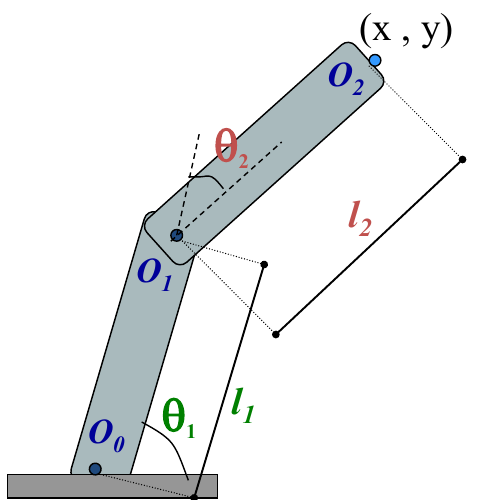
\includegraphics[width=\linewidth,height=0.51\textheight,keepaspectratio]{klimchik_l3_p013_2r.png}
        \end{column}
        \begin{column}{0.53\textwidth}
            \small
            \[
                o_0=0,\quad o_1=
                \begin{bmatrix}a_1c_1\\a_1s_1\\0\end{bmatrix},
            \]
            \[
                o_2=
                \begin{bmatrix}a_1c_1+a_2c_{12}\\a_1s_1+a_2s_{12}\\0\end{bmatrix}.
            \]
            \[
                z_0=z_1=\begin{bmatrix}0\\0\\1\end{bmatrix}.
            \]
        \end{column}
    \end{columns}
\end{frame}

\begin{frame}[t]{Column One by Cross Product}
    \framesubtitle{Crossing the vertical base axis with the tool position rotates the planar moment arm}
    \begin{columns}[T,onlytextwidth]
        \begin{column}{0.48\textwidth}
            \[
                z_0\times(o_2-o_0)=
                \begin{bmatrix}
                    -a_1s_1-a_2s_{12}\\
                    a_1c_1+a_2c_{12}\\
                    0
                \end{bmatrix}.
            \]
        \end{column}
        \begin{column}{0.48\textwidth}
            \[
                J_1=
                \begin{bmatrix}
                    -a_1s_1-a_2s_{12}\\a_1c_1+a_2c_{12}\\0\\0\\0\\1
                \end{bmatrix}.
            \]
        \end{column}
    \end{columns}
    \medskip
    The lower half is the joint axis itself, so this planar joint contributes only $\omega_z$.
\end{frame}

\begin{frame}[t]{Column Two, and the Two Routes Agree}
    \framesubtitle{The elbow moment arm contains only link 2, giving the second column directly}
    \begin{columns}[T,onlytextwidth]
        \begin{column}{0.48\textwidth}
            \[
                J_2=
                \begin{bmatrix}
                    -a_2s_{12}\\a_2c_{12}\\0\\0\\0\\1
                \end{bmatrix}.
            \]
            Its moment arm begins at the elbow origin, so link 1 does not appear.
        \end{column}
        \begin{column}{0.48\textwidth}
            Deleting the spatial rows this arm cannot move leaves
            \[
                \begin{bmatrix}
                    -a_1s_1-a_2s_{12}&-a_2s_{12}\\
                    a_1c_1+a_2c_{12}&a_2c_{12}\\
                    1&1
                \end{bmatrix}.
            \]
            It agrees entry for entry with the differentiated result.
        \end{column}
    \end{columns}
\end{frame}

\begin{frame}[t]{Differentiating the Chain Instead of the Equations}
    \framesubtitle{Replace only the elementary factor that contains the selected joint variable}
    \[
        T=T_{\mathrm{base}}\,[T_1(q)\,H(q_i)\,T_2(q)]\,T_{\mathrm{tool}}.
    \]
    \[
        T'_{q_i}=T_{\mathrm{base}}\,[T_1(q)\,H'(q_i)\,T_2(q)]\,T_{\mathrm{tool}}.
    \]
    Every other factor is untouched because it does not depend on $q_i$. One such product per joint gives all derivative matrices; this is the chain rule arranged for an implementation loop.
\end{frame}

\begin{frame}[t]{Reading a Jacobian Column out of the Derivative Matrix}
    \framesubtitle{Translation comes from the last column; angular velocity comes from a skew matrix}
    \[
        [J]_{1..3,i}=[T'_{q_i}]_{1..3,4}.
    \]
    To get the angular half, remove the current orientation:
    \[
        S(\omega)=T'_{q_i}T^{-1}
    \]
    in the upper-left $3\times3$ block. Read the vector as
    \[
        \omega_x=S_{32},\qquad\omega_y=S_{13},\qquad\omega_z=S_{21}.
    \]
\end{frame}

\begin{frame}[t]{Elementary Translations and Their Derivatives}
    \framesubtitle{A prismatic elementary transform differentiates to one fixed matrix entry}
    \[
        \frac{\partial T_x}{\partial x}=
        \begin{bmatrix}0&0&0&1\\0&0&0&0\\0&0&0&0\\0&0&0&0\end{bmatrix},\quad
        \frac{\partial T_y}{\partial y}=
        \begin{bmatrix}0&0&0&0\\0&0&0&1\\0&0&0&0\\0&0&0&0\end{bmatrix},\quad
        \frac{\partial T_z}{\partial z}=
        \begin{bmatrix}0&0&0&0\\0&0&0&0\\0&0&0&1\\0&0&0&0\end{bmatrix}.
    \]
    The derivative is independent of the translation value: it simply selects the corresponding coordinate in the last column.
\end{frame}

\begin{frame}[t]{Elementary Rotations and Their Derivatives}
    \framesubtitle{At zero angle, rotation derivatives are the embedded skew generators}
    \[
        R_x'(0)=
        \begin{bmatrix}0&0&0\\0&0&-1\\0&1&0\end{bmatrix},\quad
        R_y'(0)=
        \begin{bmatrix}0&0&1\\0&0&0\\-1&0&0\end{bmatrix},\quad
        R_z'(0)=
        \begin{bmatrix}0&-1&0\\1&0&0\\0&0&0\end{bmatrix}.
    \]
    In homogeneous-transform form, add a zero fourth row and column. These are exactly the skew generators from the infinitesimal-rotation construction; zero angle is a special case, not the general derivative.
\end{frame}

\begin{frame}[t]{Three Routes, One Jacobian}
    \framesubtitle{Choose the construction that fits the available model and the task at hand}
    \begin{columns}[T,onlytextwidth]
        \begin{column}{0.31\textwidth}
            \begin{block}{Task equations}
                Differentiate closed-form kinematics. Shortest on paper, but requires explicit task equations.
            \end{block}
        \end{column}
        \begin{column}{0.31\textwidth}
            \begin{block}{Joint axes}
                Build columns from axes and moment arms. No symbolic differentiation is needed.
            \end{block}
        \end{column}
        \begin{column}{0.31\textwidth}
            \begin{block}{Transform chain}
                Replace an elementary factor by its derivative. Mechanical and suitable for code.
            \end{block}
        \end{column}
    \end{columns}
    The first route gives an analytic Jacobian; the geometric and transform-chain routes give the geometric Jacobian. At the same configuration they are related by the representation-rate map.
\end{frame}

\begin{frame}[t]{The Inverse Differential Problem}
    \framesubtitle{Given an end-effector velocity, find joint rates that realize it}
    \[
        v=J(q)\dot q
        \qquad\Rightarrow\qquad
        \dot q=J^{-1}(q)v
    \]
    only when $J$ is square and nonsingular. Two failures are fundamental:
    \begin{itemize}
        \item near a singularity, an inverse may yield physically excessive joint rates;
        \item for a redundant robot, $J$ is rectangular and has no ordinary inverse.
    \end{itemize}
\end{frame}

\begin{frame}[t]{Inversion as a Minimum-Norm Problem}
    \framesubtitle{The pseudoinverse chooses the smallest joint-rate vector among the available solutions}
    \[
        \min\ \frac12\|\dot q\|^2
        \qquad\text{subject to}\qquad J\dot q=v.
    \]
    Its solution is
    \[
        \dot q=J^{\#}v.
    \]
    If the demand is infeasible, the same construction first minimizes the task-space error and then chooses the smallest-norm joint vector among those minimizers.
\end{frame}

\begin{frame}[t]{The Pseudoinverse}
    \framesubtitle{One unique matrix always exists; convenient product formulas require full rank}
    \small
    \[
        JJ^{\#}J=J,\quad J^{\#}JJ^{\#}=J^{\#},\quad
        (JJ^{\#})^T=JJ^{\#},\quad(J^{\#}J)^T=J^{\#}J.
    \]
    \begin{columns}[T,onlytextwidth]
        \begin{column}{0.31\textwidth}
            \begin{block}{Square, full rank}
                \[
                    J^{\#}=J^{-1}
                \]
            \end{block}
        \end{column}
        \begin{column}{0.31\textwidth}
            \begin{block}{Full row rank}
                \[
                    J^{\#}=J^T(JJ^T)^{-1}
                \]
            \end{block}
        \end{column}
        \begin{column}{0.31\textwidth}
            \begin{block}{Full column rank}
                \[
                    J^{\#}=(J^TJ)^{-1}J^T
                \]
            \end{block}
        \end{column}
    \end{columns}
    At rank deficiency, compute it from a singular-value decomposition rather than these products.
\end{frame}

\begin{frame}[t]{A Singular 2R Arm, Worked}
    \framesubtitle{At full extension the two Jacobian columns are parallel and the rank is one}
    \[
        J=
        \begin{bmatrix}-2s_1&-s_1\\2c_1&c_1\end{bmatrix},
        \qquad
        J^{\#}=\frac15
        \begin{bmatrix}-2s_1&2c_1\\-s_1&c_1\end{bmatrix}.
    \]
    Neither full-rank product formula applies. Instead, $JJ^{\#}$ and $J^{\#}J$ are symmetric and the four Penrose relations hold.
\end{frame}

\begin{frame}[t]{Feasible and Forbidden Directions}
    \framesubtitle{At a singular configuration, the pseudoinverse projects a requested velocity onto the range of $J$}
    \begin{columns}[T,onlytextwidth]
        \begin{column}{0.50\textwidth}
            \[
                J\dot q=JJ^{\#}v=v^{\perp}.
            \]
            The range of $J$ contains feasible task velocities; its orthogonal complement contains directions that no joint rate can produce.
            \[
                q_1=\pi/6:\quad
                \dot q=\begin{bmatrix}0.1\\0.05\end{bmatrix},\quad
                v^{\perp}=\begin{bmatrix}-1/8\\\sqrt3/8\end{bmatrix}.
            \]
        \end{column}
        \begin{column}{0.46\textwidth}
            \centering
            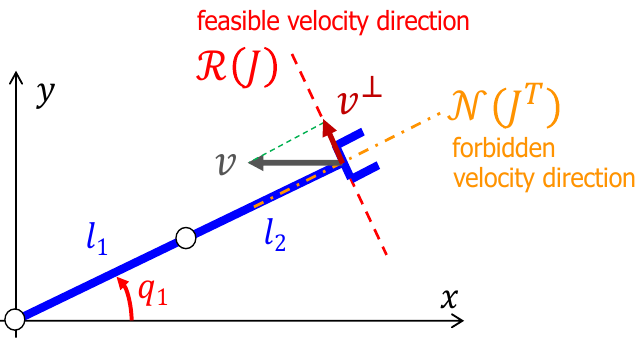
\includegraphics[width=\linewidth,height=0.54\textheight,keepaspectratio]{deluca12a_p021_ranges.png}
        \end{column}
    \end{columns}
\end{frame}

\begin{frame}[t]{Inverting at Higher Differential Order}
    \framesubtitle{Differentiating the velocity relation brings in the Jacobian rate and acceleration}
    \[
        \ddot q=J_r^{-1}(q)\left(\ddot r-\dot J_r(q)\dot q\right).
    \]
    One more product rule gives
    \[
        \dddot q=J_r^{-1}(q)
        \left(\dddot r-2\dot J_r(q)\ddot q-\ddot J_r(q)\dot q\right).
    \]
    The inverse, or a pseudoinverse when necessary, remains the leading map at each differential order. Integrating a higher-order command down produces smoother joint motion.
\end{frame}

\begin{frame}[t]{What This Leaves Open}
    \framesubtitle{The Jacobian exposes the next control and modelling questions}
    \begin{columns}[T,onlytextwidth]
        \begin{column}{0.48\textwidth}
            \begin{itemize}
                \item How can singular configurations be found and avoided?
                \item What should a redundant arm do with its unused joint-rate freedom?
            \end{itemize}
        \end{column}
        \begin{column}{0.48\textwidth}
            \begin{itemize}
                \item How does the statics duality map forces to joint torques?
                \item How should numerical conditioning near singularities be handled, including damped alternatives?
            \end{itemize}
        \end{column}
    \end{columns}
\end{frame}

\begin{frame}[t]{Reference Materials}
    \begin{itemize}
        \item A. Klimchik --- L3 Differential kinematics v01
        \item A. De Luca --- 11 DifferentialKinematics
        \item A. De Luca --- 12a InverseDifferentialKinematics
    \end{itemize}
\end{frame}


\fbckg{fibeamer/figs/last_page.png}
\frame[plain]{}

\end{document}
